\documentclass[
	classe=$1^{ere}STI2D$
]{coursclass}

\usetikzlibrary{calc,positioning}

\title{Chapitre 7 : Lois de probabilités}
\date{}

\begin{document}

\maketitle

\begin{definition}[Arbre de probabilités]
	Une expérience aléatoire peut être représentée par un \textbf{arbre de probabilités} si elle est composée de plusieurs \textit{épreuves}.

	Deux épreuves sont \textbf{indépendantes} lorsque le résultat de l'une n'influence pas la probabilité des résultats de l'autre.
\end{definition}

\begin{exemple}
	On fait une expérience qui consiste à lancer un dé équilibré 3 fois de suite, et à regarder si on a obtenu un $6$.

	On note $A$ l'évènement «Le dé est tombé sur $6$». Ainsi on peut dessiner l'arbre suivant :
	\begin{center}
		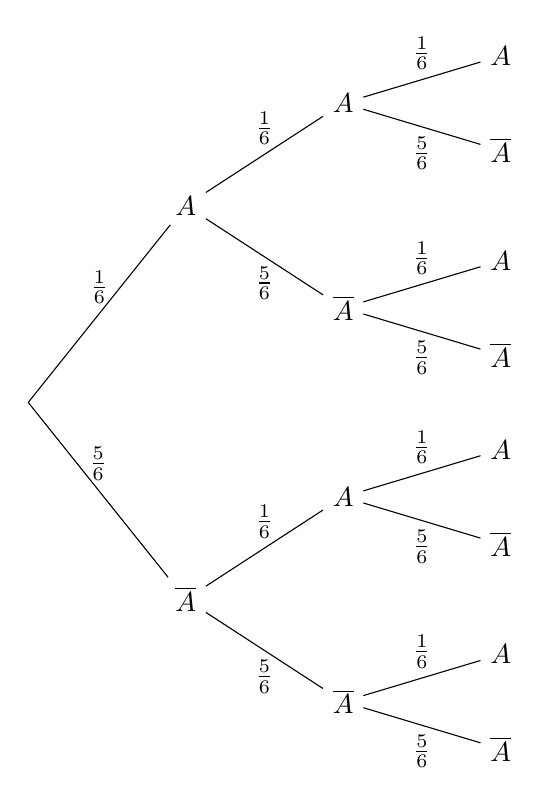
\begin{tikzpicture}
			\coordinate (START) at (0,0);
			\node (A) at (2,2.5) {$A$};
			\node (NA) at (2,-2.5) {$\overline{A}$};
			\draw (START) -- node[above] {$\frac{1}{6}$} (A)
			(START) -- node[above] {$\frac{5}{6}$} (NA);
			\foreach \n in {A,NA} {
					\node (Ab) at ($(\n) + (2,1.3)$) {$A$};
					\node (NAb) at ($(\n) + (2,-1.3)$) {$\overline{A}$};
					\draw (\n) -- node[above] {$\frac{1}{6}$} (Ab);
					\draw (\n) -- node[below] {$\frac{5}{6}$} (NAb);
					\foreach \nb in {Ab,NAb} {
							\node (Ac) at ($(\nb) + (2,0.6)$) {$A$};
							\node (NAc) at ($(\nb) + (2,-0.6)$) {$\overline{A}$};
							\draw (\nb) -- node[above] {$\frac{1}{6}$} (Ac);
							\draw (\nb) -- node[below] {$\frac{5}{6}$} (NAc);
						}
				}
		\end{tikzpicture}
	\end{center}
\end{exemple}

\begin{propriete}[Probabilité d'une issue]
	Si les épreuves que représente notre arbre sont indépendantes, la probabilité d'une issue est le \textbf{produit} des probabilités du chemin qui mène à cette issue.
\end{propriete}

\begin{exemple}
	Dans l'exemple précédent, l'issue «On a obtenu un  six \textit{uniquement} au premier lancé» est représentée par le chemin $(A, \overline{A}, \overline{A})$. Sa probabilité est alors $\dfrac{1}{6} × \dfrac{5}{6} × \dfrac{5}{6} = \dfrac{25}{216}$.
\end{exemple}

\begin{propriete}[Probabilité d'un évènement]
	La probabilité d'un évènement est la somme des probabilités des issues qui forment cet évènement.
\end{propriete}

\begin{exemple}
	Si on veut obtenir la probabilité d'obtenir \textit{exactement} $1$ six sur les trois lancés : 

	Cet évènement est constitué des issues $(A, \overline{A}, \overline{A})$, $(\overline{A}, A, \overline{A})$ et $(\overline{A}, \overline{A}, A)$. Sa probabilité est donc

	\begin{center}
		\begin{tikzpicture}
			\coordinate (START) at (0,0);
			\node (A) at (2,2.5) {$A$};
			\node (NA) at (2,-2.5) {$\overline{A}$};
			\draw (START) -- node[above] {$\frac{1}{6}$} (A)
			(START) -- node[above] {$\frac{5}{6}$} (NA);
			\foreach \n in {A,NA} {
					\node (Ab) at ($(\n) + (2,1.3)$) {$A$};
					\node (NAb) at ($(\n) + (2,-1.3)$) {$\overline{A}$};
					\draw (\n) -- node[above] {$\frac{1}{6}$} (Ab);
					\draw (\n) -- node[below] {$\frac{5}{6}$} (NAb);
					\foreach \nb in {Ab,NAb} {
							\node (Ac) at ($(\nb) + (2,0.6)$) {$A$};
							\node (NAc) at ($(\nb) + (2,-0.6)$) {$\overline{A}$};
							\draw (\nb) -- node[above] {$\frac{1}{6}$} (Ac);
							\draw (\nb) -- node[below] {$\frac{5}{6}$} (NAc);
						}
				}
				\coordinate (TEMP) at (6,0.6);
				\node[right=of TEMP] {→ issue $(A, \overline{A}, \overline{A})$, probabilité $\dfrac{1}{6} × \dfrac{5}{6} × \dfrac{5}{6} = \dfrac{25}{216}$};
				\coordinate (TEMP) at (6,-1.8);
				\node[right=of TEMP] {→ issue $(\overline{A}, A, \overline{A})$, probabilité $\dfrac{5}{6} × \dfrac{1}{6} × \dfrac{5}{6} = \dfrac{25}{216}$};
				\coordinate (TEMP) at (6,-3.2);
				\node[right=of TEMP] {→ issue $(\overline{A}, \overline{A}, A)$, probabilité $\dfrac{5}{6} × \dfrac{5}{6} × \dfrac{1}{6} = \dfrac{25}{216}$};
		\end{tikzpicture}

		$$ \dfrac{25}{216} + \dfrac{25}{216} + \dfrac{25}{216} = \dfrac{75}{216} = \dfrac{25}{72} $$
	\end{center}
\end{exemple}

\end{document}